\begin{figure}[H]
	\begin{center}
		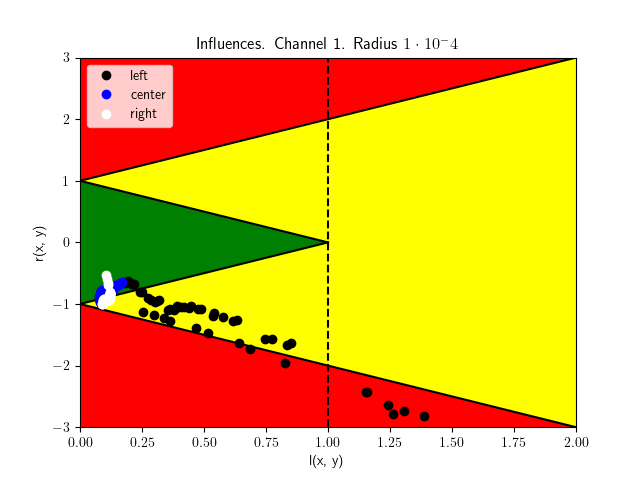
\includegraphics[scale=0.77]{status_ch1_rad1}
		\label{pic:ch11}
		\caption{Диаграмма статусов. Канал 1. Радиус интервала $1 \cdot 10 ^ {-4}$}
	\end{center}
\end{figure}

Для этого случая покажем диаграмму рассеяния, отметим на ней коридор совместных зависимостей и выбросы:

\begin{figure}[H]
	\begin{center}
		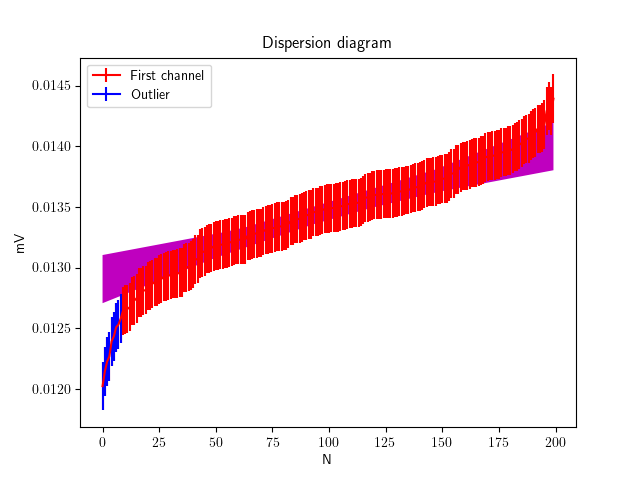
\includegraphics[scale=0.77]{dispd}
		\label{pic:d1}
		\caption{Диаграмма рассеяния. Канал 1. Радиус интервала $1 \cdot 10 ^ {-4}$}
	\end{center}
\end{figure}

\begin{figure}[H]
	\begin{center}
		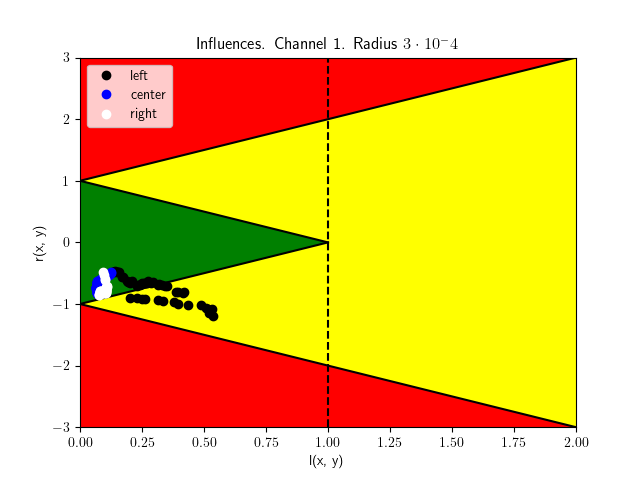
\includegraphics[scale=0.83]{status_ch1_rad3}
		\label{pic:ch13}
		\caption{Диаграмма статусов. Канал 1. Радиус интервала $3 \cdot 10 ^ {-4}$}
	\end{center}
\end{figure}

\begin{figure}[H]
	\begin{center}
		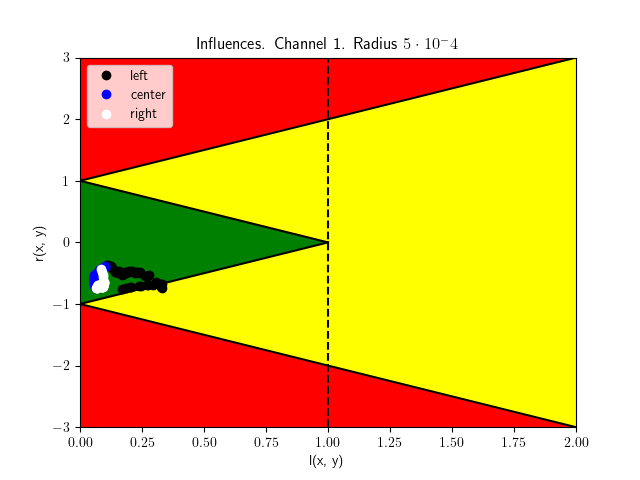
\includegraphics[scale=0.83]{status_ch1_rad5}
		\label{pic:ch15}
		\caption{Диаграмма статусов. Канал 1. Радиус интервала $5 \cdot 10 ^ {-4}$}
	\end{center}
\end{figure}

\begin{figure}[H]
	\begin{center}
		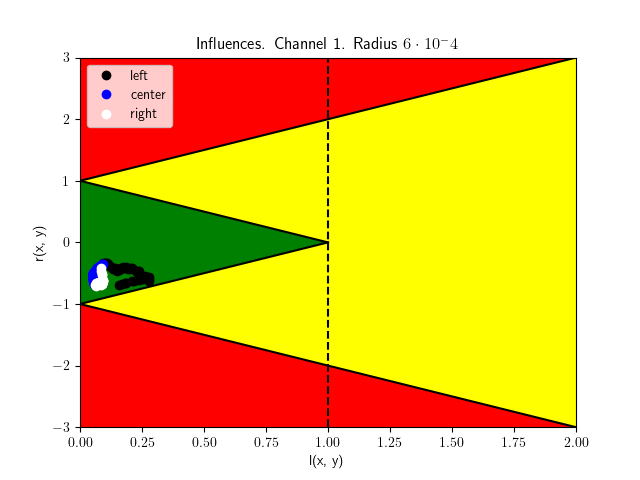
\includegraphics[scale=0.83]{status_ch1_rad6}
		\label{pic:ch16}
		\caption{Диаграмма статусов. Канал 1. Радиус интервала $6 \cdot 10 ^ {-4}$}
	\end{center}
\end{figure}

\begin{figure}[H]
	\begin{center}
		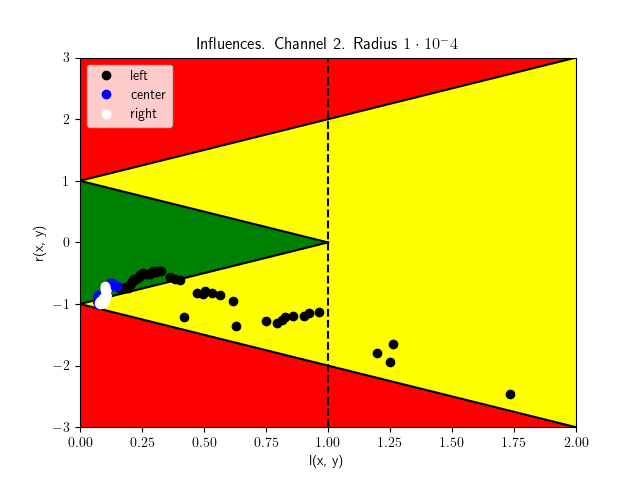
\includegraphics[scale=0.83]{status_ch2_rad1}
		\label{pic:ch21}
		\caption{Диаграмма статусов. Канал 2. Радиус интервала $1 \cdot 10 ^ {-4}$}
	\end{center}
\end{figure}

\begin{figure}[H]
	\begin{center}
		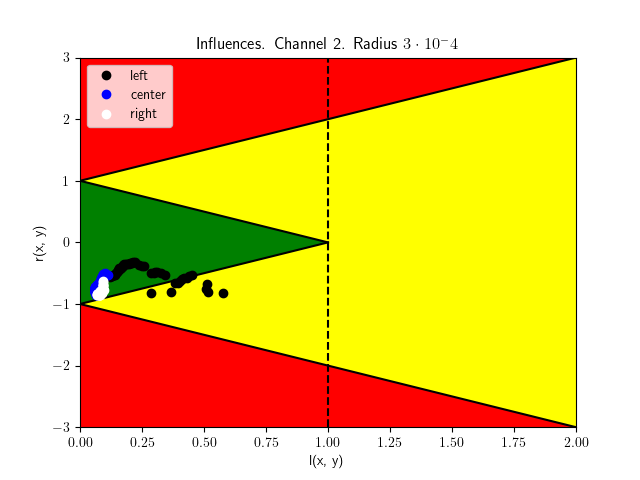
\includegraphics[scale=0.83]{status_ch2_rad3}
		\label{pic:ch23}
		\caption{Диаграмма статусов. Канал 2. Радиус интервала $3 \cdot 10 ^ {-4}$}
	\end{center}
\end{figure}

\begin{figure}[H]
	\begin{center}
		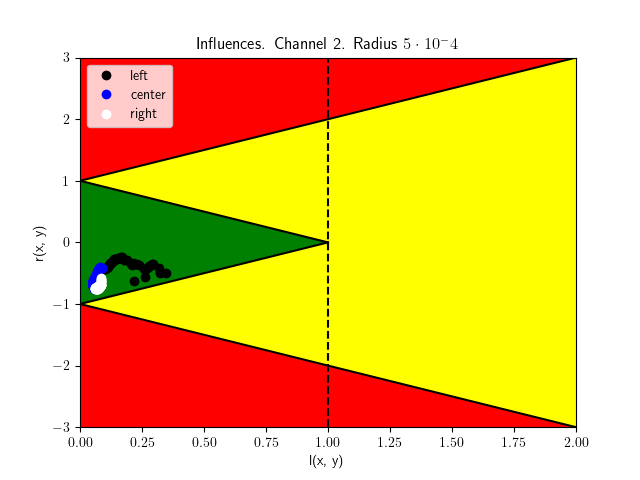
\includegraphics[scale=0.83]{status_ch2_rad5}
		\label{pic:ch25}
		\caption{Диаграмма статусов. Канал 2. Радиус интервала $5 \cdot 10 ^ {-4}$}
	\end{center}
\end{figure}

\begin{figure}[H]
	\begin{center}
		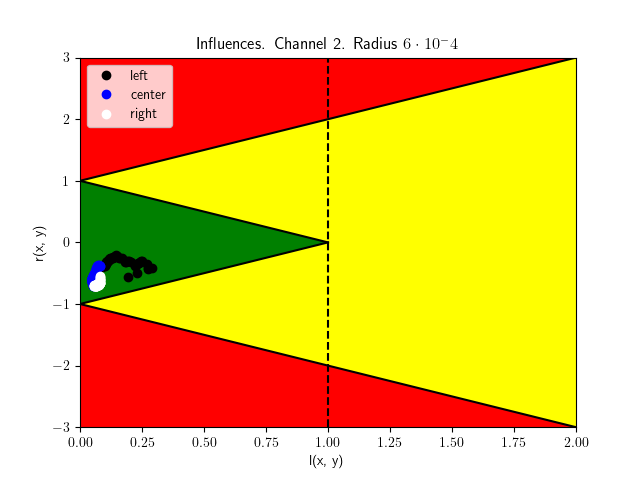
\includegraphics[scale=0.83]{status_ch2_rad6}
		\label{pic:ch26}
		\caption{Диаграмма статусов. Канал 2. Радиус интервала $6 \cdot 10 ^ {-4}$}
	\end{center}
\end{figure}